
\subsection{Seq2SeqBiLSTM}
La classe \texttt{Seq2SeqBiLSTM} implementa un'architettura simile al modello Seq2SeqLSTM, ma i layer LSTM dell'encoder sono bidirezionali.\\

\subsubsection{Encoder}
L'encoder è composto da:
\begin{itemize}
    \item \textbf{Layer di embedding}
    \item \textbf{Un layer LSTM bidirezionale} con:
        \begin{itemize}
            \item Dimensione latente fissa
            \item Dropout del 40\%
            \item Recurrent dropout del 40\%
        \end{itemize}
    \item \textbf{Layer di Concatenazione}: Concatena gli stati del layer LSTM bidirezionale
\end{itemize}

\subsubsection{Decoder}
Il decoder include:
\begin{itemize}
    \item \textbf{Layer di embedding}
    \item \textbf{Layer LSTM}:
        \begin{itemize}
            \item Dimensione latente pari \(2 * \textit{dimensione\_latente\_fissa}\), per adattarsi alla concatenazione degli stati provenienti dall'encoder.
            \item Dropout del 40\%
            \item Recurrent dropout del 20\%
        \end{itemize}
    \item \textbf{Layer di attenzione}
    \item \textbf{Layer di Concatenazione}
    \item \textbf{Layer denso di output}
\end{itemize}

Di seguito, possiamo vedere un diagramma dell'architettura del modello Seq2SeqBiLSTM nella figura \ref{fig:seq2seqbilstm_model_architecture}.

\begin{figure}[H]
    \centering
    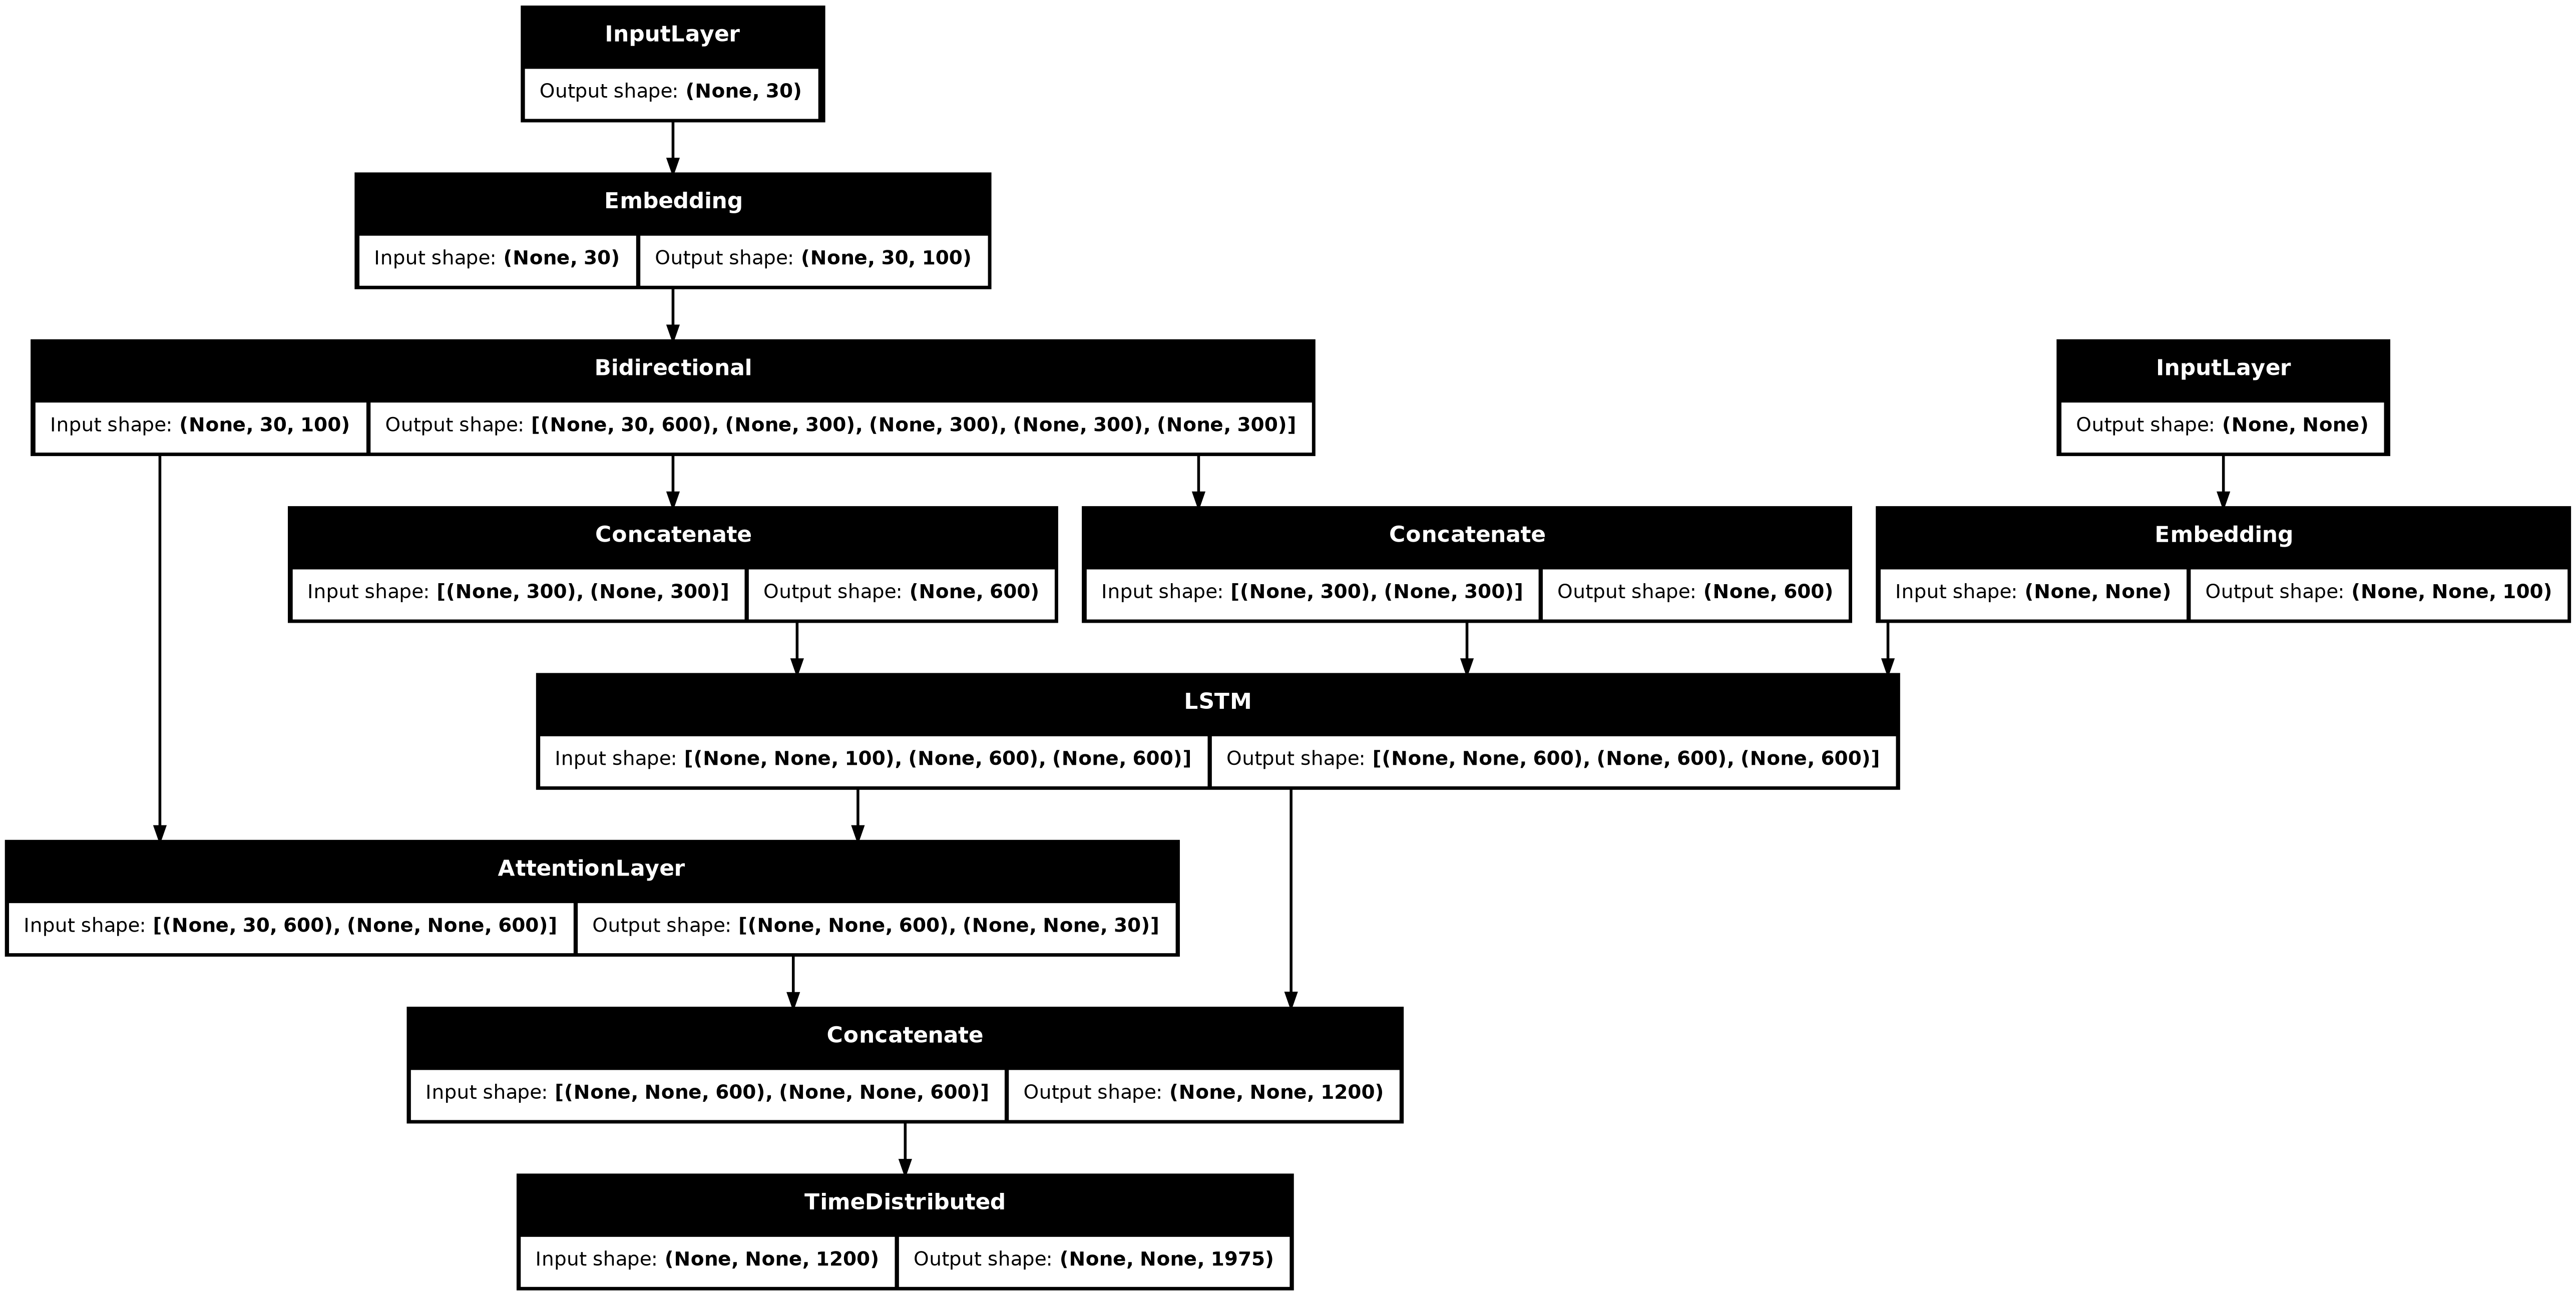
\includegraphics[width=1\textwidth]{media/Seq2SeqBiLSTM_image.png}
    \caption{Diagramma dell'architettura del modello Seq2SeqBiLSTM}
    \label{fig:seq2seqbilstm_model_architecture}
\end{figure}

\training{Adam}{50}
\risultati{DA INSERIRE}{DA INSERIRE}{DA INSERIRE}{DA INSERIRE}

\begin{figure}[H]
    \centering
    %TODO: Aggiungere immagine traingin loss È DA AGGIORNARE
    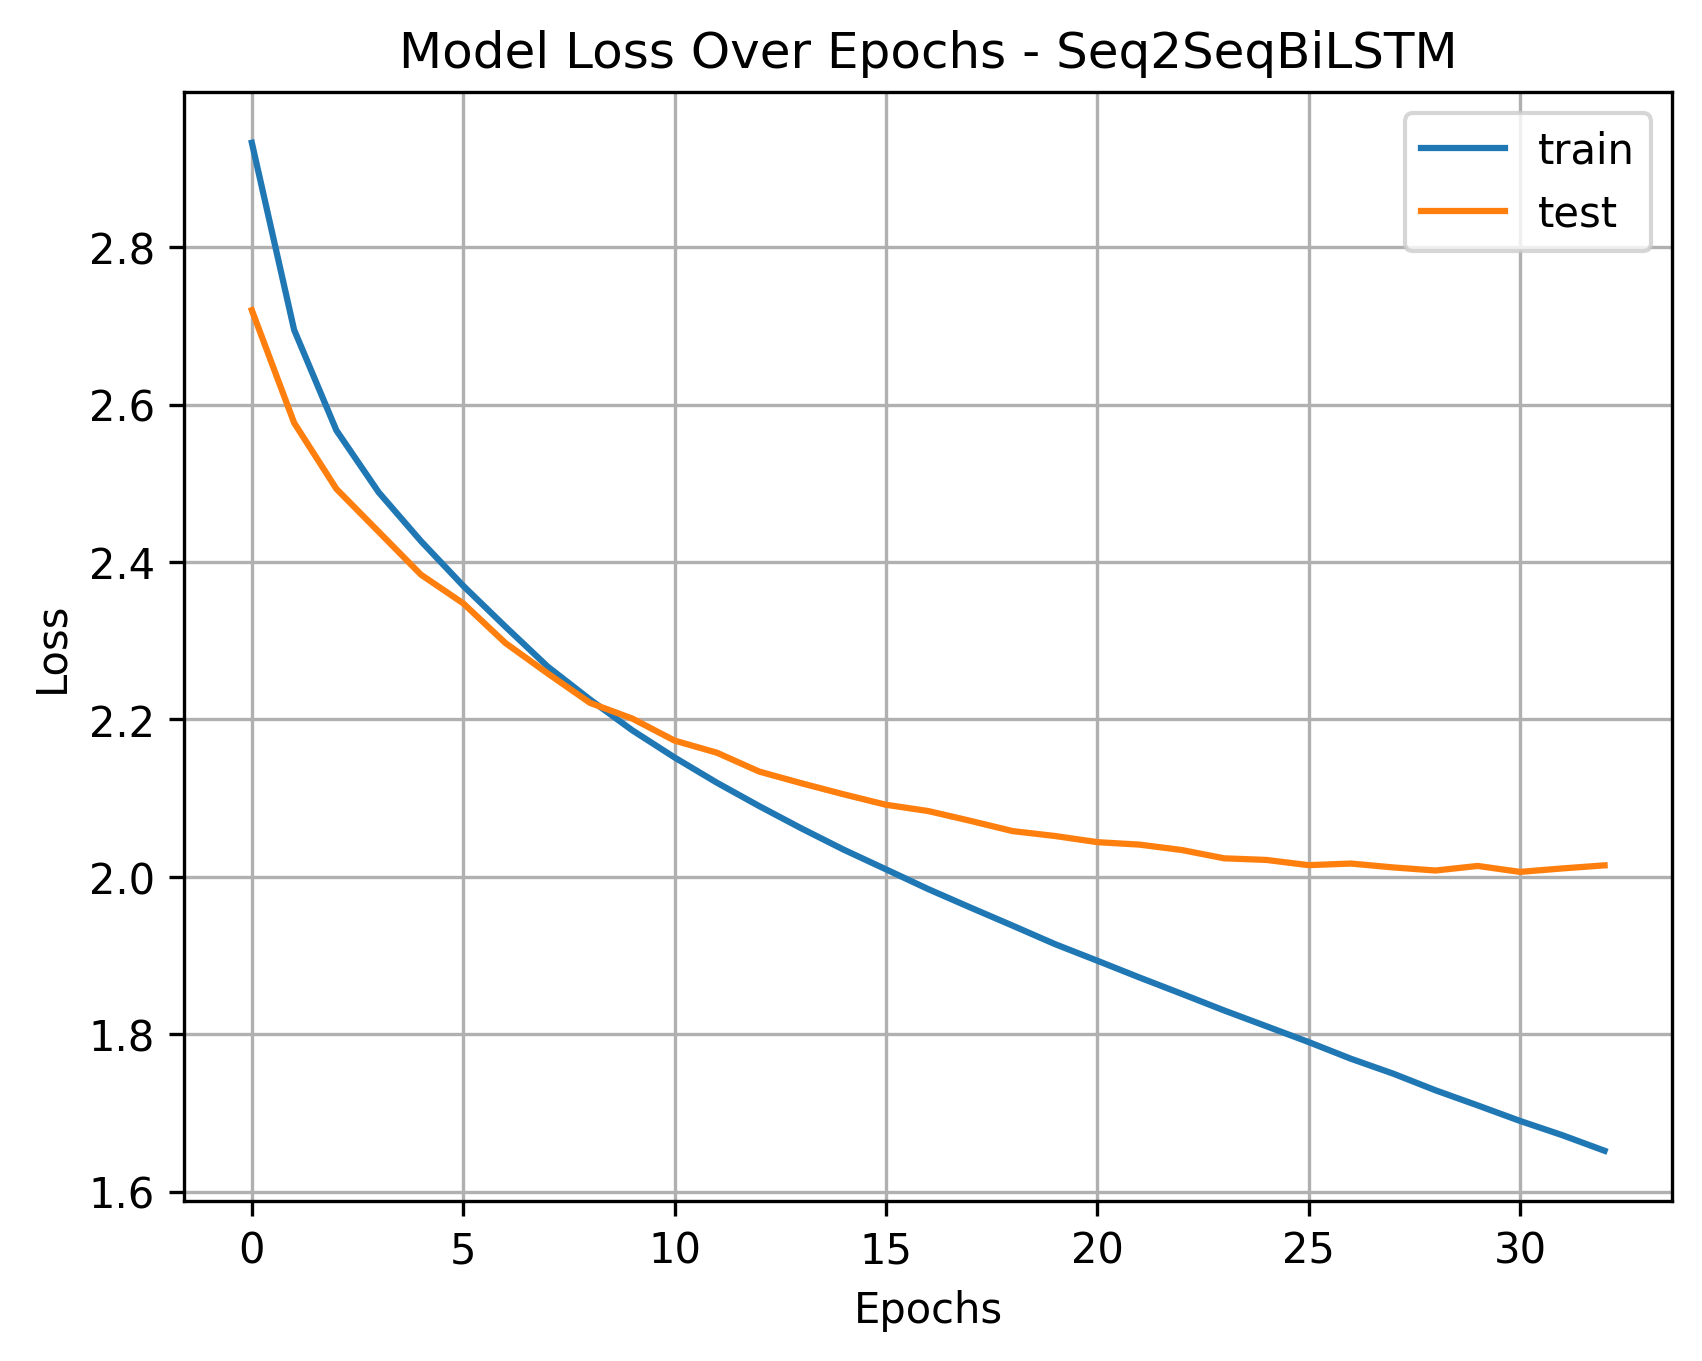
\includegraphics[width=0.75\textwidth]{media/Seq2SeqBiLSTM_originale_lossplot.png}
    \caption{Andamento delle loss durante l'addestramento}
    \label{fig:seq2seqbilstm_loss_plot}
\end{figure}
